\documentclass{beamer}
\usepackage[utf8]{inputenc}
\usepackage[T1]{fontenc}
\usepackage{lmodern}
\usepackage[english]{babel}
\usepackage{lsfolien}
\usepackage{hyperref}

\myfootline{System Modelling and Semantic Web}{Carsten Lehmann}

\title{Problem Solving Tools - Trimming
	\vskip1em}

\subtitle{Modul Systemmodellierung und Semantisches Web}

\author{Carsten Lehmann}

\date{21. Juni 2022}


\begin{document}

	\begin{frame}[plain]
		\maketitle
	\end{frame}

	\section{Überblick über das Thema}
	
	\begin{frame}{Was ist Trimmen?}
		\begin{columns}
			\column{.4\textwidth}
			\begin{itemize}
				\item Der Wandel in der Automobilindustrie vom Händler zum Direktvertrieb
				\item Lean Management (effiziente Gestaltung der Wertschöpfungskette)
				\item System on a chip (statt vieler einzelner Komponenten)
			\end{itemize}
			\column{.6\textwidth}
			\begin{figure}
				\centering
			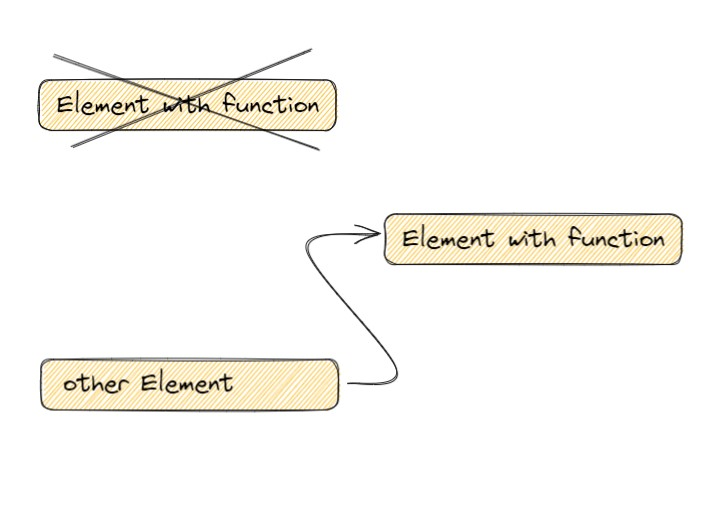
\includegraphics[width=.7\textwidth]{img/Intro.jpg}
				\caption{Trimming Principle}
			\end{figure}	
		\end{columns}
		Viele Prozesse und Produkte folgen dem Trend des Trimmens. Oft, um Kosten zu sparen, während die gleiche Funktion beibehalten wird.
	\end{frame}
	
	\begin{frame}{Def. of Trimming}
		Mit dem Problemlösungswerkzeug Trimming wird versucht, ein System so zu vereinfachen, dass die gleiche oder eine bessere Funktion gewährleistet ist, aber Elemente des Systems entfernt werden können.
	\end{frame}
	
	\begin{frame}{Kurzer Überblick über den Inhalt}
		\begin{itemize}
			\item Grundregeln des Trimmwerkzeugs
			\item Voraussetzungen für die Verwendung von Trimming
			\item Fallstudie
		\end{itemize}
	\end{frame}
	
	\begin{frame}{Inhalt Details}
		\begin{itemize}
			\item Basic Regeln für das Trimmwerkzeug und Systemverbesserungen
    		\begin{itemize}
    			\item für physikalische Elemente in einem System
    			\item für Prozesse
    		\end{itemize}
			\item Voraussetzungen für das Trimming
    		\begin{itemize}
    			\item Funktionserfassung
    			\item Tests für tragfähiges System
    			\item Bewältigung von Situationen, in denen Elemente funktional gekoppelt sind
    		\end{itemize}
			\item Fallstudie für ein System:
    		\begin{itemize}
    			\item Beispiel für das Trimmen an einem Produkt
    		\end{itemize}
		\end{itemize}
	\end{frame}
	
	\section{Grundregeln des Trimmwerkzeugs und Systemverbesserungen}
	
	\begin{frame}{Das Trimmwerkzeug}
	Das System muss vor dem Trimmen sehr gut bekannt sein. \\
	Hauptziel des Trimmens: Entfernen unnötiger Elemente aus einem System
		\begin{itemize}
			\item Warum beseitigen wir nicht dieses Element?
			\begin{itemize}
    			\item Brauchen wir die nützliche(n) Funktion(en), die dieses Element erfüllt?
    			\item Kann stattdessen eines der anderen Elemente des Systems die nützliche(n) Funktion(en) erfüllen?
    			\item Könnten wir eines der anderen Elemente ändern, um die nützliche(n) Funktion(en) zu erfüllen?
    			\item Gibt es ein Element oder eine Ressource in der Umgebung des Systems, das/die die Funktion(en) ausführen kann?
    			\item Gibt es ein Element oder eine Ressource in der Umgebung des Systems, das/die verändert werden könnte, um die Funktion zu erfüllen?
    			\item Können wir die Funktion(en) durch die Kombination anderer Elemente und Ressourcen erfüllen?
		    \end{itemize}
		\end{itemize}
	\end{frame}
	
	
	\begin{frame}{Das Trimming - Werkzeug}
		\begin{block}{Warum beseitigen wir nicht dieses Element?}
			Die Fragen werden von oben nach unten geprüft. Wenn Fragen weiter oben positiv beantwortet werden können, führt dies in der Regel zu einer idealeren Lösung.
		\end{block}
	\end{frame}
	
	
	\begin{frame}{Trimming Question 1/6}
		\begin{columns}
			\column{.6\textwidth}
		Brauchen wir die nützliche(n) Funktion(en), die dieses Element erfüllt?
		
		Hinweis: FAA Funktionen Atribute Analyse
		\begin{itemize}
			\item Hat das Element überhaupt eine nützliche Funktion? (sichtbar in der FAA)
			\item Bestimmen Sie, ob die nützlichen Funktionen tatsächlich benötigt werden
			\item Element darf keine anderen nützlichen Aufgaben im System erfüllen
			\item Das Element darf die Funktionalität des Systems in zukünftigen Szenarien nicht beeinträchtigen.
		\end{itemize}
			\column{.4\textwidth}
			\begin{figure}
				\centering
				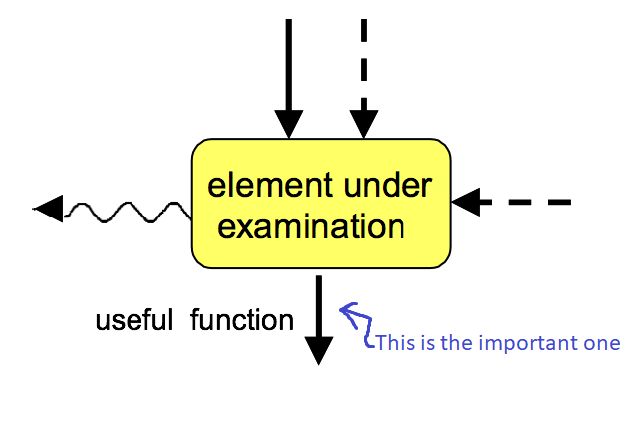
\includegraphics[width=1.1\textwidth]{img/q1.png}
				\caption{Nützliche ausgehende Funktionen bestimmen, ob das Element getrimmt werden kann}
			\end{figure}	
		\end{columns}
	\end{frame}
	
	\begin{frame}{Trimming Question 2/6}
		Kann stattdessen eines der anderen Elemente die Funktion übernehmen?
		\begin{itemize}
			\item Könnten andere Elemente im FAA-Modell die Funktion des Elements übernehmen, das wir kürzen wollen?
			\item Bestimmen Sie, ob die nützlichen Funktionen tatsächlich benötigt werden
			\item Beginnen Sie mit den Elementen, die am engsten mit dem beschnittenen Teil verbunden sind.
			\item arbeiten Sie sich von dort aus zu den Elementen im Modell vor, die am weitesten von dem Element entfernt sind
		\end{itemize}
	\end{frame}
	
	
	\begin{frame}{Trimming Question 3/6}
		Können wir eines der anderen Elemente ändern, um die nützliche(n) Funktion(en) zu erfüllen?
		\begin{itemize}
			\item Können wir ein Element ändern, um die Funktion auszuführen?
			\item Hierfür ist es sinnvoll, den Entwicklungsstand der jeweiligen Elemente zu analysieren.
			\item Beginnen Sie mit den Elementen, die sich am wenigsten entwickelt haben
			\item von dort aus weiter zu Elementen mit weniger evolution Potenzial arbeiten
		\end{itemize}
		
		Siehe nächste Seite...
	\end{frame}
	
	\begin{frame}{Trimming Question 3/6}
	Können wir eines der anderen Elemente ändern, um die nützliche(n) Funktion(en) zu erfüllen?
		\begin{figure}
			\centering
			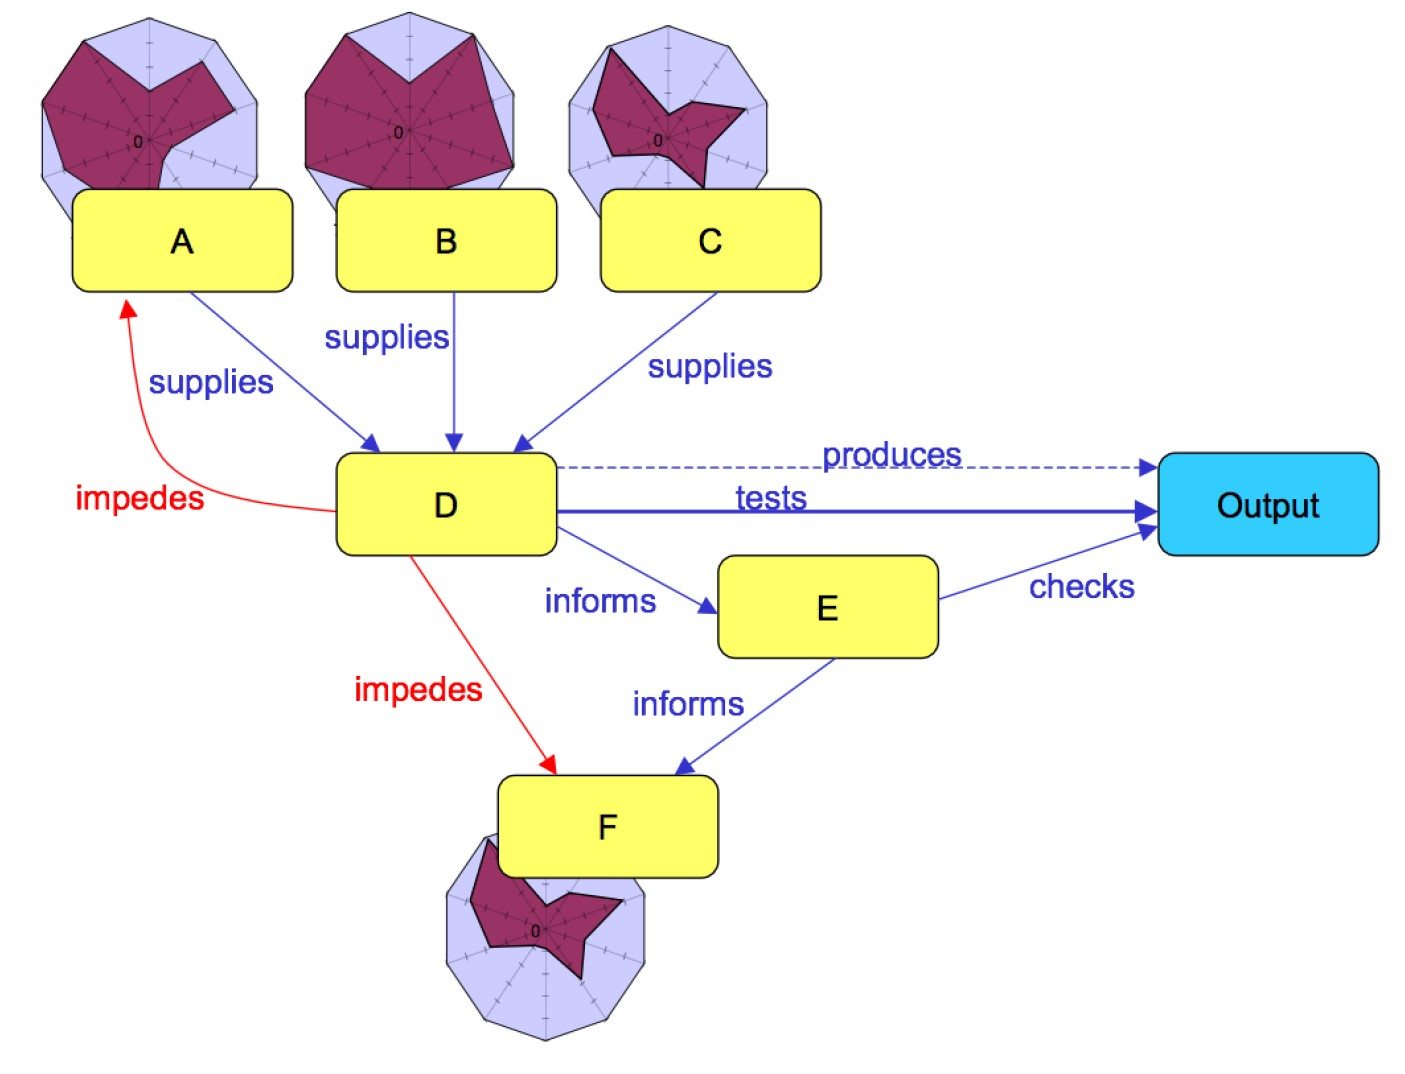
\includegraphics[width=0.6\textwidth]{img/q3.jpg}
			\caption{Entwicklungspotenzial-Radarplots für Elemente im FAA-Modell}
		\end{figure}
	\end{frame}
	
	\begin{frame}{Trimming Question 4/6}
		Gibt es in der Umgebung des Systems ein Element oder eine Ressource, die die Funktion(en) ausführen kann?
		\begin{itemize}
			\item außerhalb des Systems nach einer Ressource suchen, die die Funktion des Elements direkt erfüllt
			\item Problem-/Chancen-Explorer-Analyse -> gibt es ein brauchbares Element in dieser Liste? 
			\item Checklisten für Ressourcen: allgemeiner Ansatz
			\item besonderes Augenmerk auf die Kategorie der "kostengünstigen Ressourcen" richten
		\end{itemize}
	\end{frame}
	
	
	\begin{frame}{Trimming Question 5/6}
		Gibt es ein Element oder eine Ressource in der Umgebung des Systems, das/die geändert werden könnte, um die Funktion(en) auszuführen?
		\begin{itemize}
			\item nach ungenutztem evolutionärem Potenzial in Elementen oder Ressourcen außerhalb
			\item Wenn eine Ressource von außen entwickelt wird, könnte sie dann die erforderliche Aktion durchführen?
		\end{itemize}
	\end{frame}
	
	\begin{frame}{Trimming Question 6/6}
		Kann ich die Funktion(en) durch die Kombination mit anderen Elementen und Ressourcen erfüllen?
		\begin{itemize}
			\item Kombination zwischen zwei oder mehreren bestehenden Elementen
			\item Kombination zwischen einem bestehenden Element und einer oder mehreren externen Ressourcen
			\item Kombination zwischen zwei oder mehreren externen Ressourcen
		\end{itemize}
	\end{frame}
	

	\begin{frame}{Trimming für Prozesse}
		Die Fragen sind im Wesentlichen dieselben wie oben, nur auf Prozesse angewandt.
		\begin{itemize}
			\item Brauchen wir die nützliche(n) Funktion(en), die dieser Prozessschritt erfüllt?
			\item Kann einer der anderen Schritte im Prozess stattdessen die nützliche(n) Funktion(en) erfüllen?
			\item Könnten wir einen der anderen bestehenden Prozessschritte ändern, um die nützliche(n) Funktion(en) auszuführen?
			\item Können wir einen neuen, einfacheren Prozessschritt einführen, der die Funktion(en) erfüllen kann?
			\item Können wir einen Prozessschritt aus einem anderen bestehenden System ändern, um die Funktion auszuführen?
			\item Können wir die Funktion(en) durch die Kombination anderer Prozessschritte erfüllen?
		\end{itemize}
	\end{frame}
	
	
	\section{Reihenfolge des Trimmings}
	
	\begin{frame}{Trimming Sequence}
		Bestimmte Leitlinien für die Anwendung des Beschneidens, aber sie sagen uns nicht, welche Elemente in welcher Reihenfolge beschnitten werden können.\\
		Die Regeln hierfür sind noch nicht vollständig oder verallgemeinerbar, aber es gibt vier nützliche Leitlinien:
		\begin{itemize}
			\item Elemente mit der höchsten Anzahl von unerwünschten Funktionen, die mit ihnen verbunden sind, sind ein Hauptkandidat für das Trimmen
			\item die Elemente mit dem höchsten Wert bieten den größten Nutzen beim Trimmen
			\item die höchsten Elemente in der Funktionshierarchie sollten vorrangig behandelt werden
			\item Elemente, die die geringste Anzahl nützlicher Funktionen bieten
		\end{itemize}
	\end{frame}
	
	\section{Trimming – Das große Ganze}

	\begin{frame}{Trimming – Das große Ganze}
		Es gibt 3 Aspekte, die wichtig sind, um zu prüfen, ob überhaupt getrimmt werden sollte:
		\begin{itemize}
			\item[a)] Funktionserfassung
            \item[b)] tests ob systeme trangfähig sind
            \item[c)] Bewältigung von Situationen, in denen Elemente funktional gekoppelt sind
		\end{itemize}
	\end{frame}

	\begin{frame}{a) Funktionserfassung}
		\begin{itemize}
			\item Erfassen Sie alle in einem System vorhandenen Funktionen so gründlich und vollständig wie möglich
			\item FAA sollte umfassend sein und vorzugsweise von mehr als einer Person validiert werden
			\item absolut sicher sein, dass ALLE nützlichen Funktionspfeile erfasst werden, die vom Element weg zeigen
		\end{itemize}
	\end{frame}

	\begin{frame}{b) viable system tests}
    	Das Viable System Model (VSM) nach Stafford Beer beschreibt 5 notwendige Bedingungen für die Lebensfähigkeit eines Systems:
		\begin{itemize}
			\item Implementation (Wertschöpfende Aktivitäten)
			\item Co-ordination (Koordination der wertschöpfenden Systeme)
			\item Intelligence  (Zukunftsanalyse und -planung, Umwelt des Gesamtsystems)
			\item Control (Strukturen und Kontrollen für Systeme)
			\item Policy (Oberste Entscheidungseinheit)
		\end{itemize}
	\end{frame}
	
	\begin{frame}{b) viable system tests}
		\begin{block}{Implementation (Wertschöpfende Aktivitäten)}
			definiert als die Teile des Systems, die für die Durchführung der Haupttätigkeiten verantwortlich sind und dann in Teilsysteme unterteilt werden können, die wiederum als lebensfähiges System betrachtet werden 
		\end{block}
		\begin{block}{Co-ordination (Koordination der wertschöpfenden Systeme)}
			Die einzelnen Elemente und das System müssen miteinander kommunizieren. Je mehr sie dies tun und je weniger von oben aufgezwungen wird, desto autonomer funktionieren die Elemente oder Teilsysteme.
		\end{block}
	\end{frame}
	
	\begin{frame}{b) viable system tests}
		\begin{block}{Intelligence  (Zukunftsanalyse und -planung, Umwelt des Gesamtsystems)}
			Ist die wechselseitige Verknüpfung zwischen der primären Aktivität des Systems und seiner Umwelt. Dies ermöglicht die Anpassung an zukünftige, sich ändernde Umwelteinflüsse.
		\end{block}
		\begin{block}{Control (Strukturen und Kontrollen für Systeme)}
			Im VSM definiert als die (wechselseitige) Kommunikation zwischen Untereinheit und Metaebene.
		\end{block}
		\begin{block}{Policy (Oberste Entscheidungseinheit)}
			Die Richtlinienfunktion sorgt für den Abschluss des Systems als Ganzes, indem sie die allgemeine Richtung, die Werte und den Zweck der Organisationseinheit festlegt.
		\end{block}
	\end{frame}
	
	
	\begin{frame}{b) viable system tests}
		Der springende Punkt: Wenn man versucht, eines dieser wesentlichen Elemente aus einem System zu entfernen, muss man einen Ersatz für sie finden, da das System ohne sie nicht lebensfähig ist.
	\end{frame}
	
	\begin{frame}{c) Bewältigung von Situationen, in denen Elemente funktional gekoppelt sind}
		Die Komplexität eines Systems nimmt mit der Zeit zu und wird dann auch immer mehr optimiert. Die Komplexität eines Systems ist nicht gleichzusetzen mit der Anzahl der Elemente. Hohe Komplexität kann auch durch wenige Elemente mit vielen Funktionen erzeugt werden.\\
		\vspace{\baselineskip}
		Das Trimmen darf niemals die sich selbst erhaltende Fähigkeit des Systems gefährden.\\
		\vspace{\baselineskip}
		Wichtige Fragen vor dem Ausschneiden eines Elements aus dem System:
		\begin{itemize}
			\item Gibt es gekoppelte Funktionen?
			\item Gibt es Aspekte des zu beschneidenden Elements, die unser System mit dem System auf der nächsthöheren Ebene in der Hierarchie verbinden?
		\end{itemize}
		Wenn die Antwort auf eine der beiden Fragen "ja" lautet, sollte das Beschneiden nur mit Vorsicht erfolgen.
	\end{frame}
	
	
		
	\begin{frame}{Beispiel}
		\begin{figure}
			\centering
			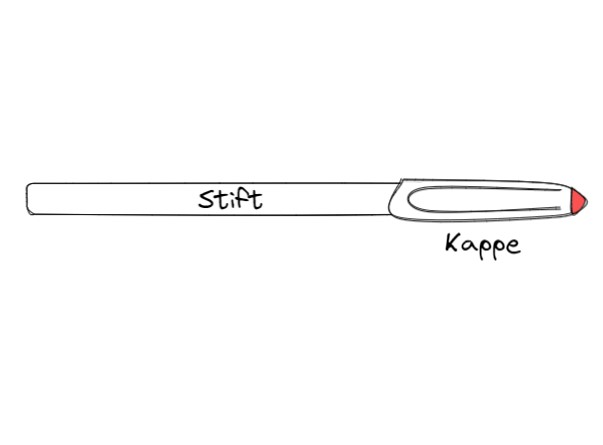
\includegraphics[width=0.6\textwidth]{img/ex.jpg}
			\caption{Beispiel für das Trimming an einem Produkts (www.michael-patra.de)}
		\end{figure}
	\end{frame}
	
	\begin{frame}{References}
		\begin{itemize}
			\item[1] Darell L. Mann. Hands-on systematic innovation for Business and Management. IFR Press, 2014
		\end{itemize}
	\end{frame}

\end{document}
